\documentclass[main.tex]{subfiles}


\begin{document}
	\section{Úvod do prostředí Robot Mesh studio}

	Našeho robota budeme programovat v prostředí Robot Mesh studio, které je zdarma dostupné na~webové stránce \href{https://www.robotmesh.com/studio}{https://www.robotmesh.com/studio}. Robota lze přes toto prostředí programovat v několika jazycích, my si pro tuto učebnici vystačíme s jazykem Blocky.

	\subsection{Vytváření nového projektu}
	K tomu, aby s prohlížečem (ve kterém budeme robota programovat) robot komunikoval, je potřeba nainstalovat do prohlížeče addon. Aktuálně je dostupný pouze pro \href{https://addons.mozilla.org/en-US/firefox/addon/robot-mesh-connect/}{FireFox} a \href{https://chrome.google.com/webstore/detail/robot-mesh-connect-app/mapfkcmnklanficcnnjkgeneakedmjkp}{Google Chrome}.

	Po nainstalování addonu přejdeme na stránku \href{https://www.robotmesh.com/studio}{https://www.robotmesh.com/studio}:

	\begin{figure}[h!]
		\centering
		\fbox{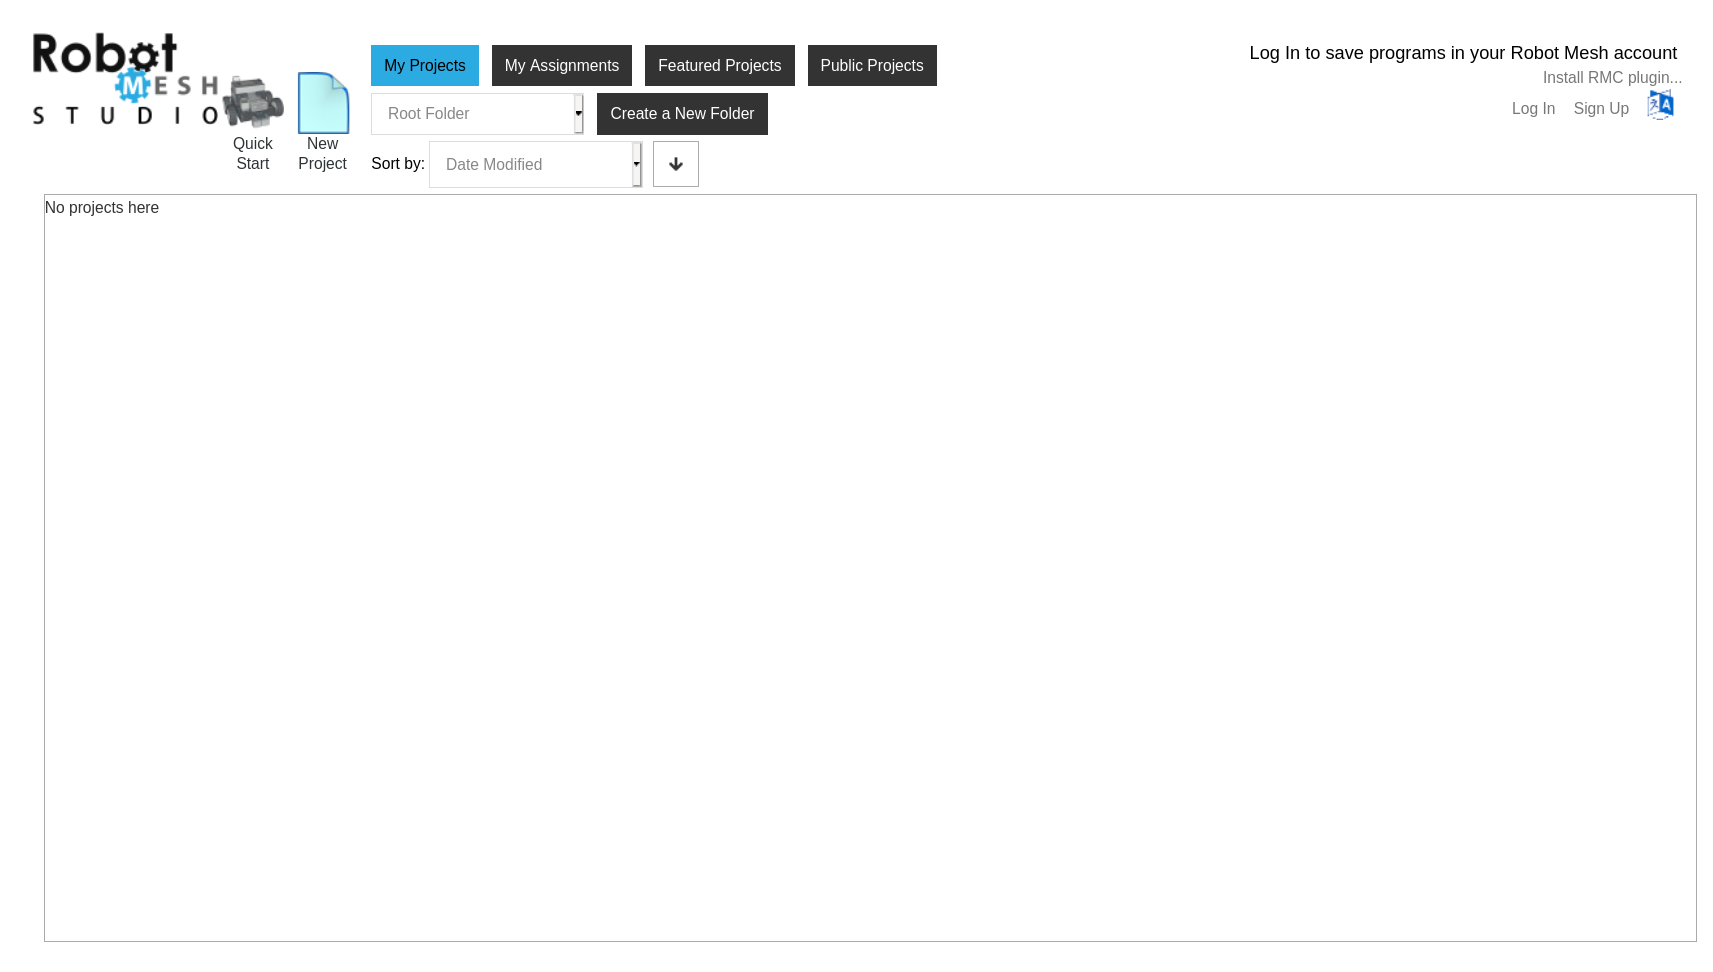
\includegraphics[width=0.85\linewidth]{Images/01/default-robotmesh-website.png}}
	\end{figure}

	K vytvoření nového projektu stačí kliknout na \textbf{New Project} a poté:

	\begin{figure}[h!]%
		\begin{subfigure}[t]{.3\textwidth}%
			\centering%
			\fbox{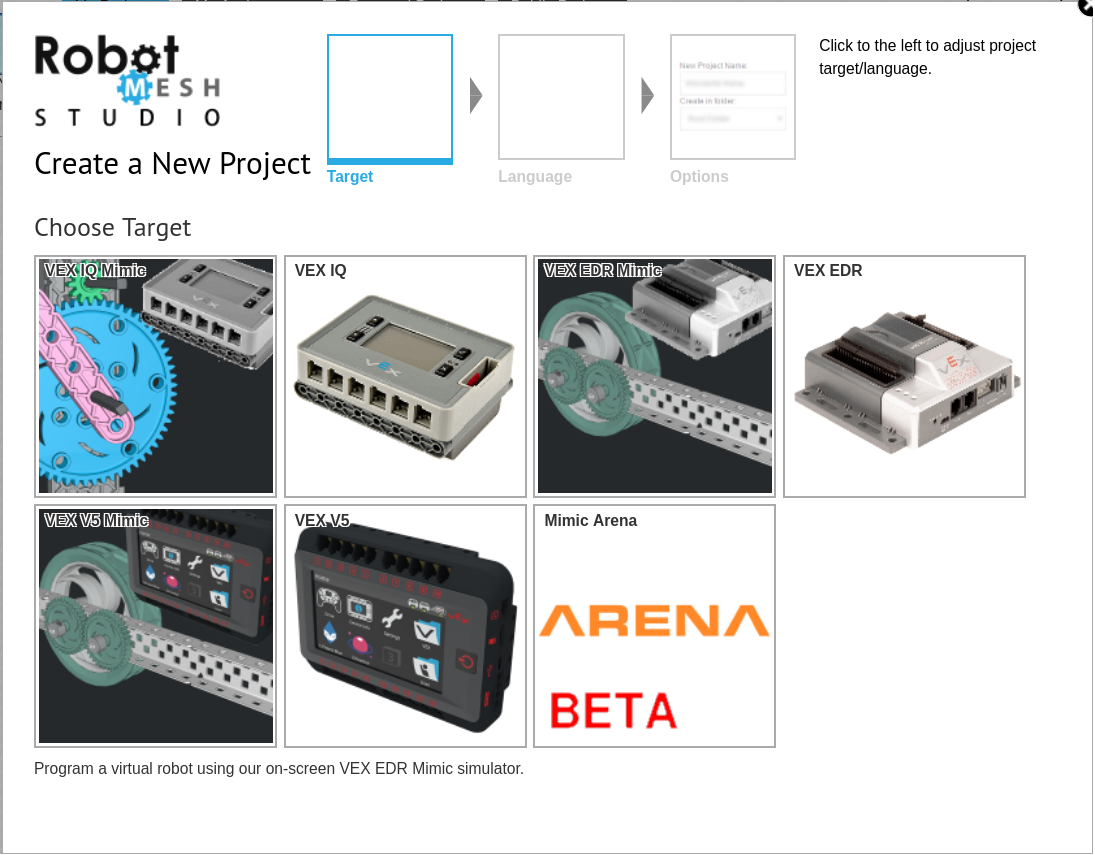
\includegraphics[width=\linewidth]{Images/01/create-project-1.png}}%
			\caption{kliknout na \textbf{VEX V5}}%
		\end{subfigure} \hspace{.045\textwidth}%
		\begin{subfigure}[t]{.3\textwidth}%
			\centering%
			\fbox{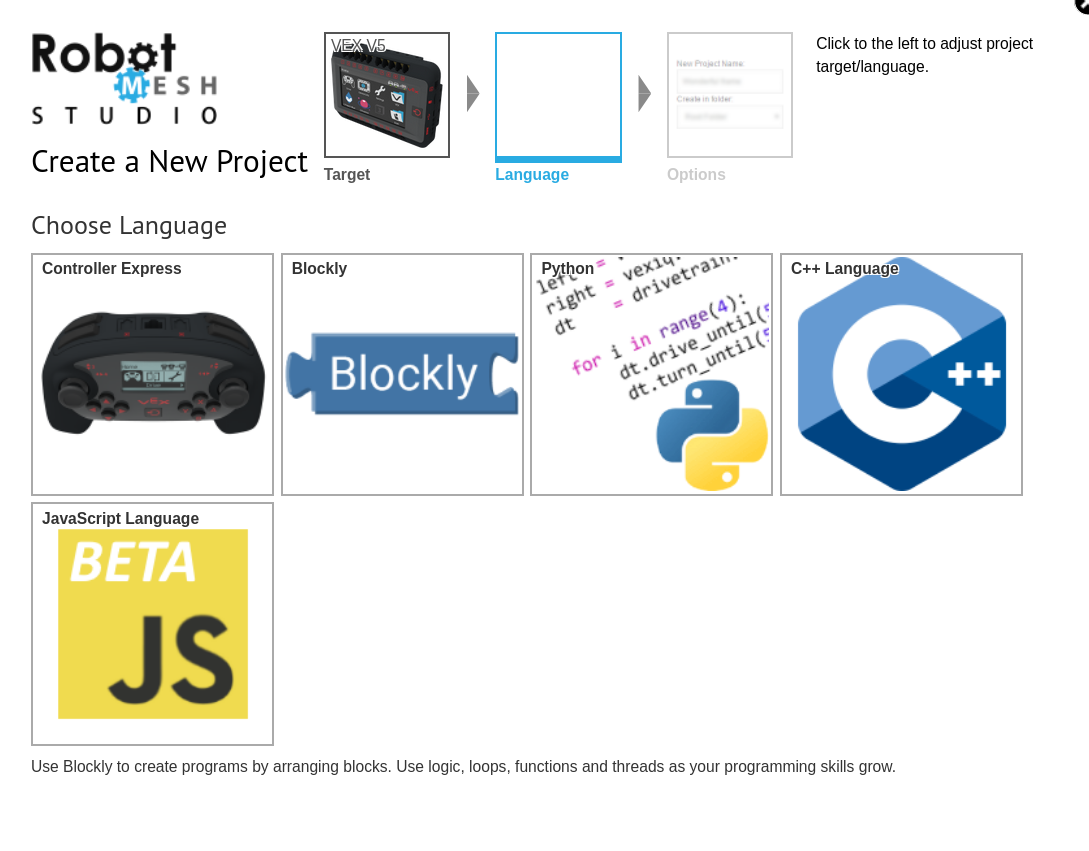
\includegraphics[width=\linewidth]{Images/01/create-project-2.png}}
			\caption{kliknout na \textbf{Blocky}}%
		\end{subfigure} \hspace{.045\textwidth}%
		\begin{subfigure}[t]{.3\textwidth}%
			\centering%
			\fbox{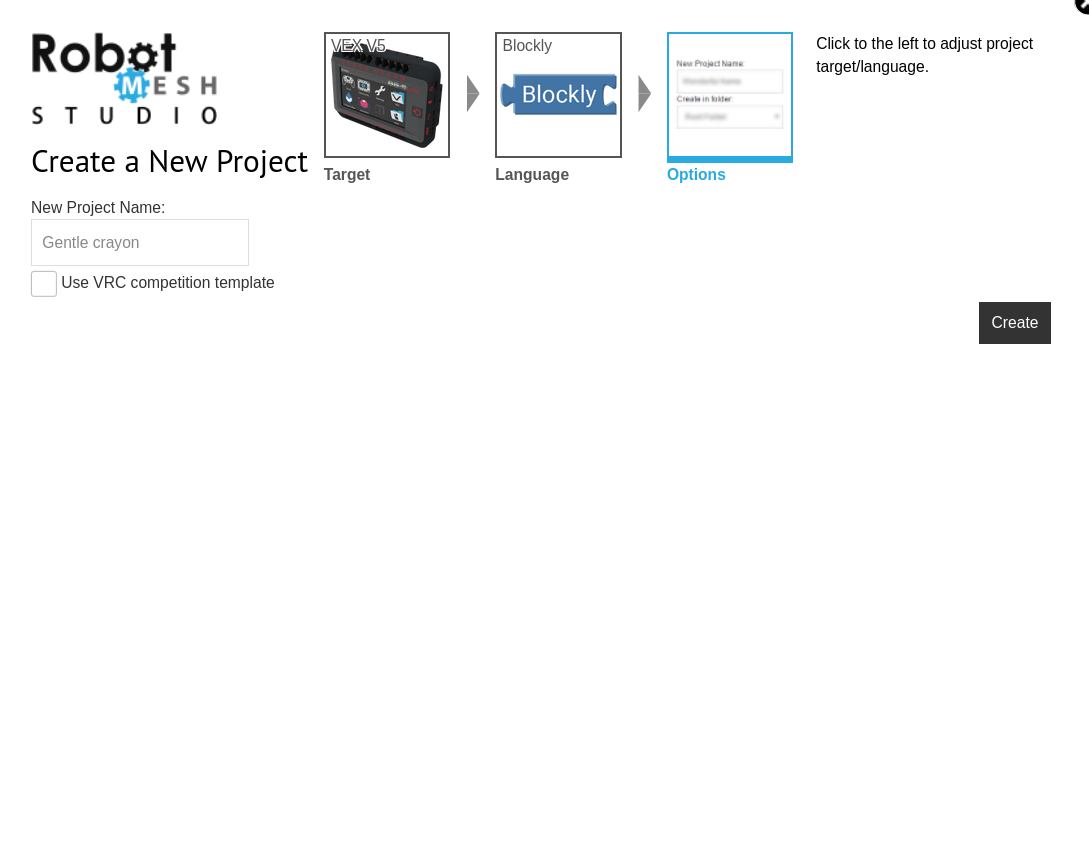
\includegraphics[width=\linewidth]{Images/01/create-project-3.png}}%
			\caption{kliknout na \textbf{Create} (případně změnit jméno projektu)}%
		\end{subfigure}%
	\end{figure}

	\newpage

	Nyní se nacházíme v samotném Robot Mesh studiu. Skládá se z několika částí:

	\begin{itemize}
		\item \textbf{Horní (ovládací) část} -- slouží ke spouštění, pozastavování a zastavování programu.
		\item \textbf{Levá (příkazová) část} -- obsahuje příkazy k ovládání robota.
		\item \textbf{Pravá (hardwarová) část} -- obsahuje nastavení motorů/senzorů (hardwaru).
		\item \textbf{Prostřední (programová) část} -- obsahuje samotný program.
		\item \textbf{Dolní (statusová) část} -- zobrazuje chybové hlášky/oznámení o běhu programu.
	\end{itemize}

	\begin{figure}[h!]
		\centering
		\fbox{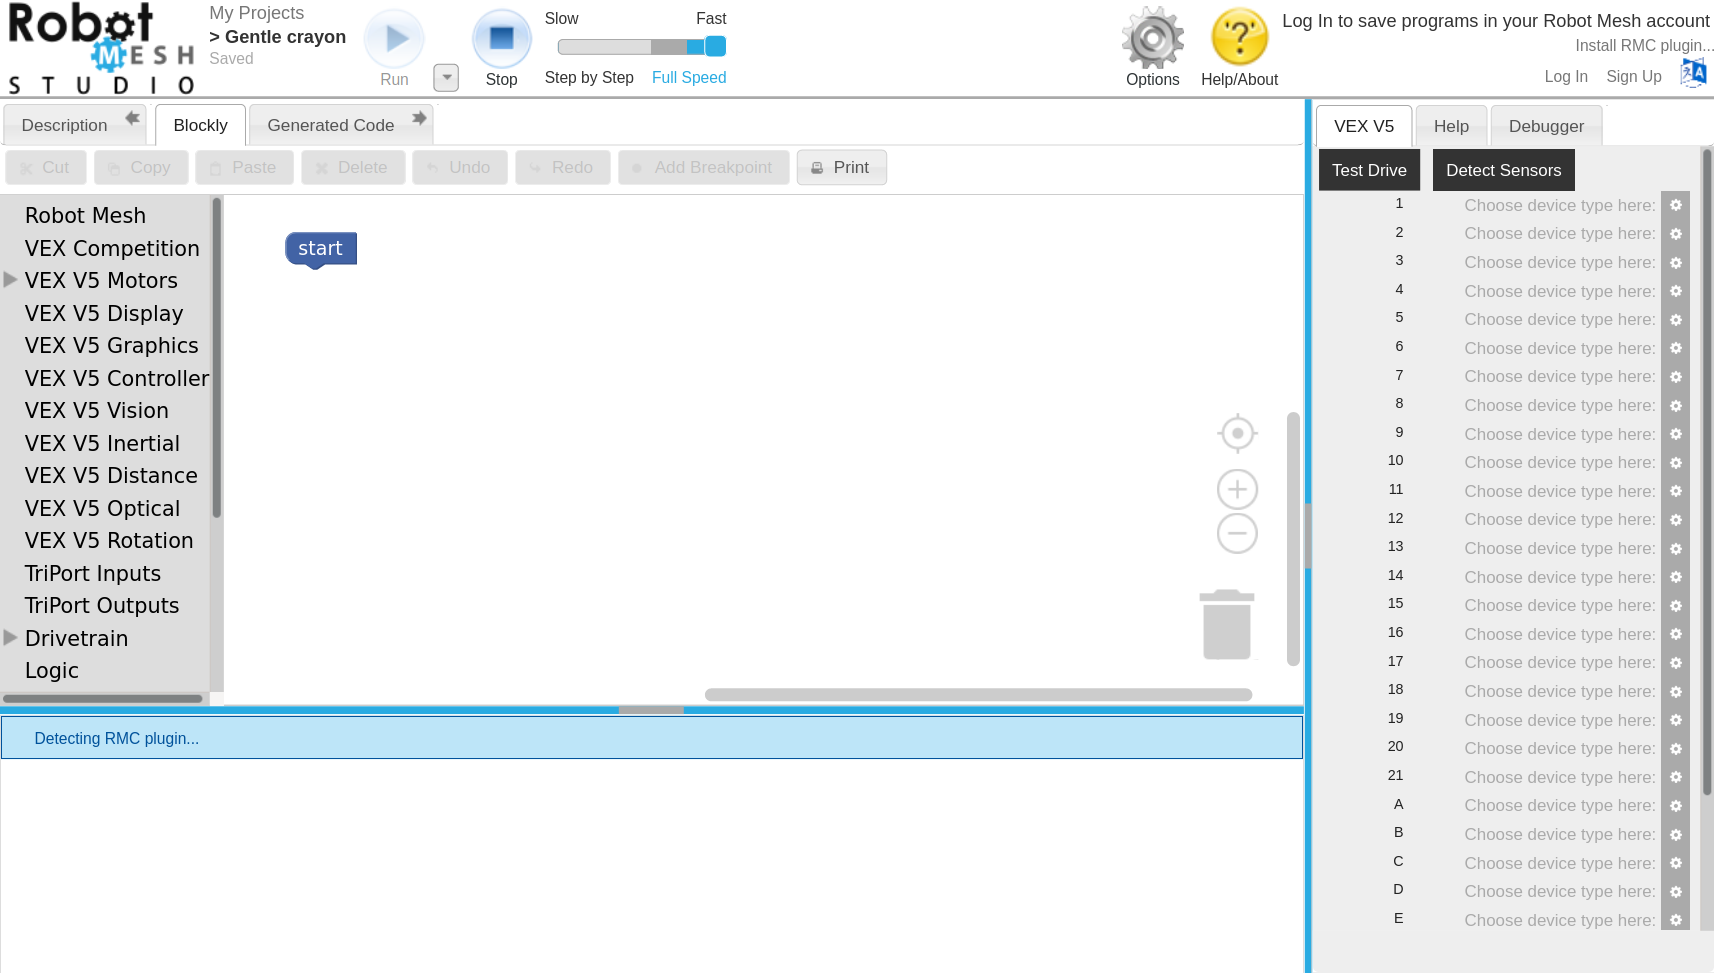
\includegraphics[width=0.85\linewidth]{Images/01/default-robotmesh-studio.png}}
	\end{figure}

	\begin{question}
		Vytvořte si nový projekt s nějakým zajímavým jménem.
	\end{question}

	\subsection{Nastavení robota}
	Zapněte robota, přes USB ho připojte k počítači a obnovte okno -- text \textit{Detecting RMC plugin...} by~měl zmizet. Je také možné, že se místo této zprávy objeví požadavek na updatování firmwaru robota. Ten můžete odkliknout a počkat, než se update nainstaluje.

	Před tím, než robota začneme programovat, je potřeba nastavit motory. Na našem robotu by motory podvozku měly být připojeny k portům $1$ a $10$ -- v hardwarové části tedy klikněte na \centerimage{\baselineskip}{Images/ui/gear.png} napravo od~čísla \textbf{1} a poté:

	\begin{figure}[h!]%
		\begin{subfigure}{.3\textwidth}%
			\centering%
			\fbox{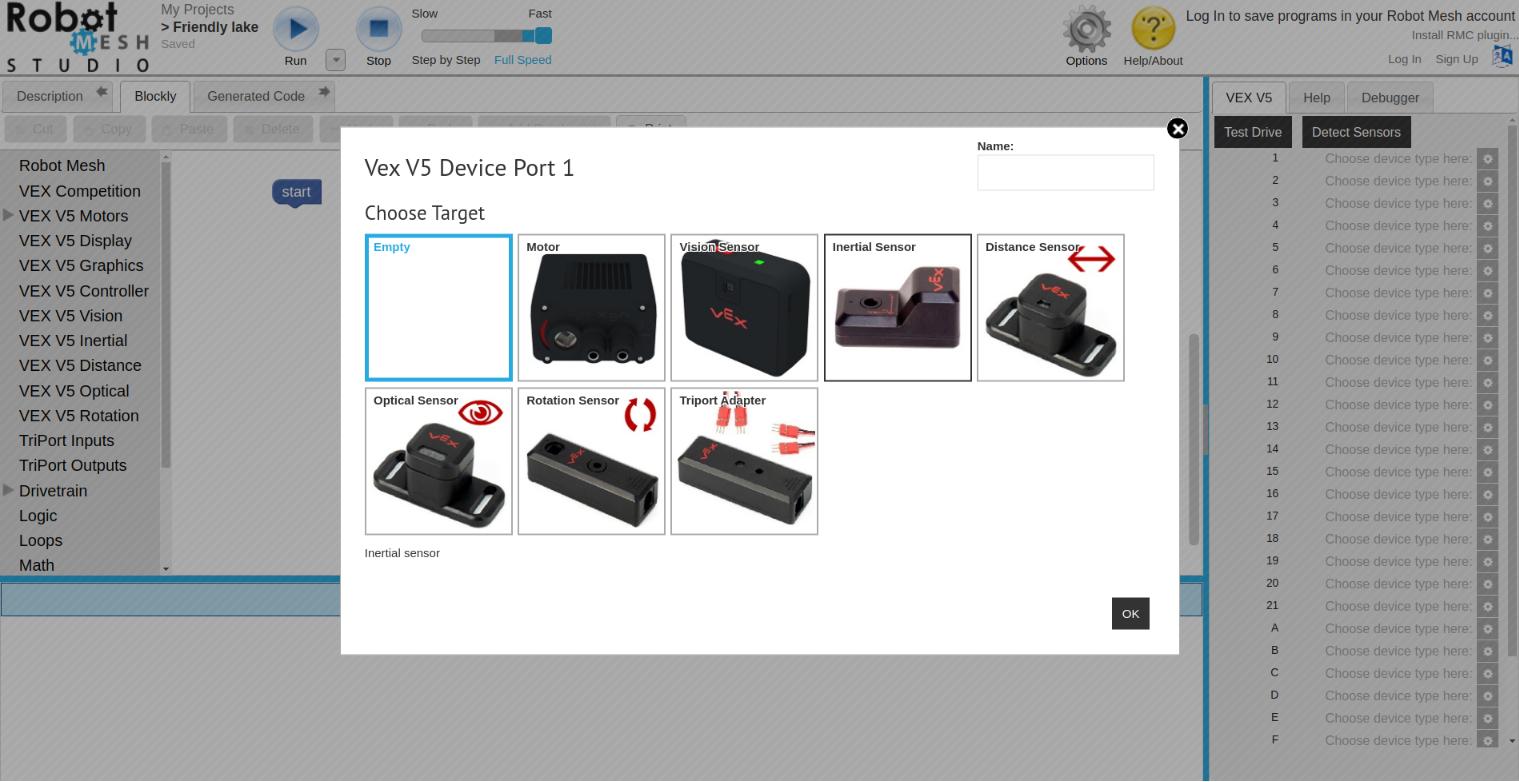
\includegraphics[width=\linewidth]{Images/01/add-motors-1.png}}%
			\caption{vyberte \textbf{motor}}%
		\end{subfigure} \hspace{.045\textwidth}%
		\begin{subfigure}{.3\textwidth}%
			\centering%
			\fbox{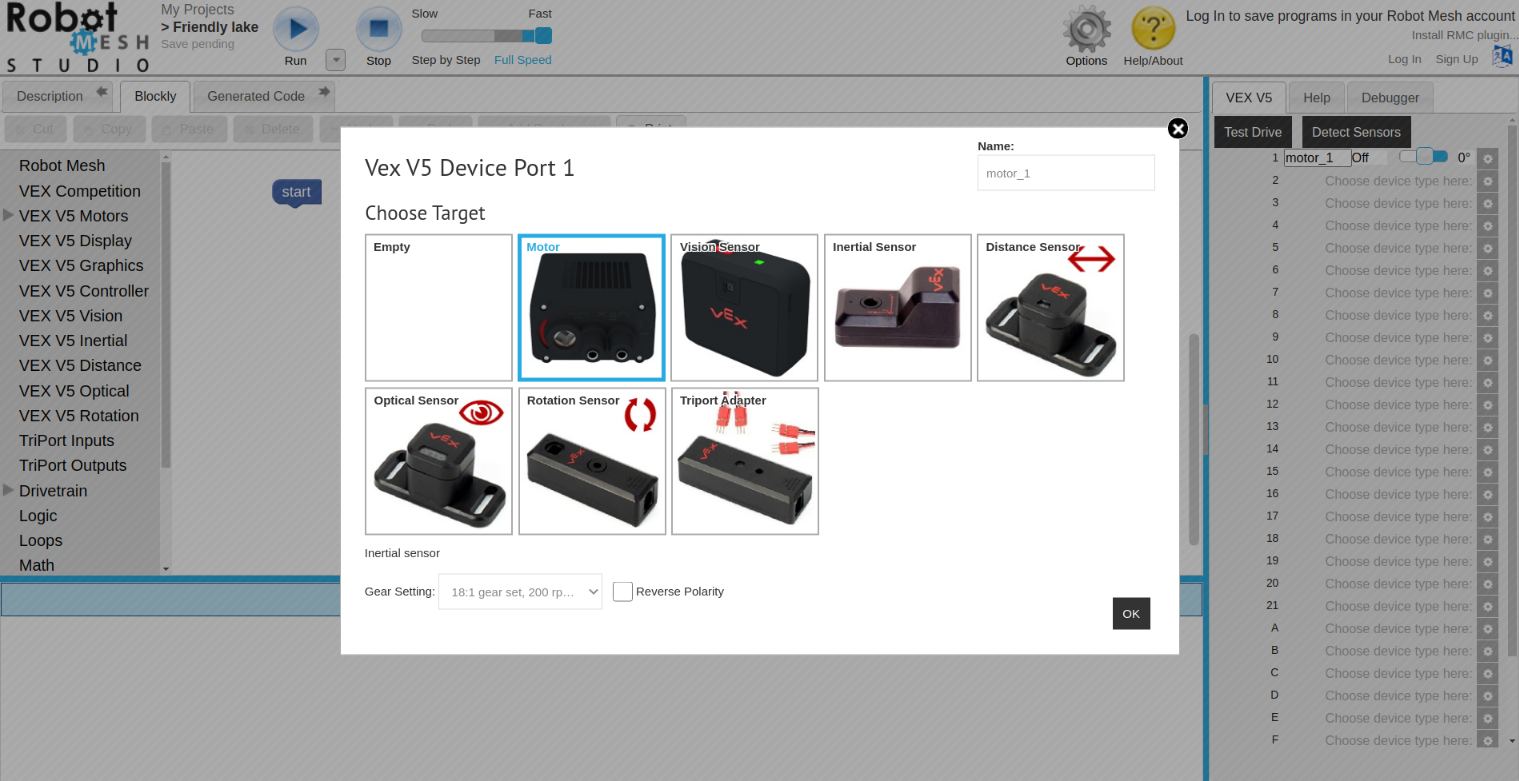
\includegraphics[width=\linewidth]{Images/01/add-motors-2.png}}
			\caption{klikněte na \textbf{OK}}%
		\end{subfigure} \hspace{.045\textwidth}%
		\begin{subfigure}{.3\textwidth}%
			\centering%
			\fbox{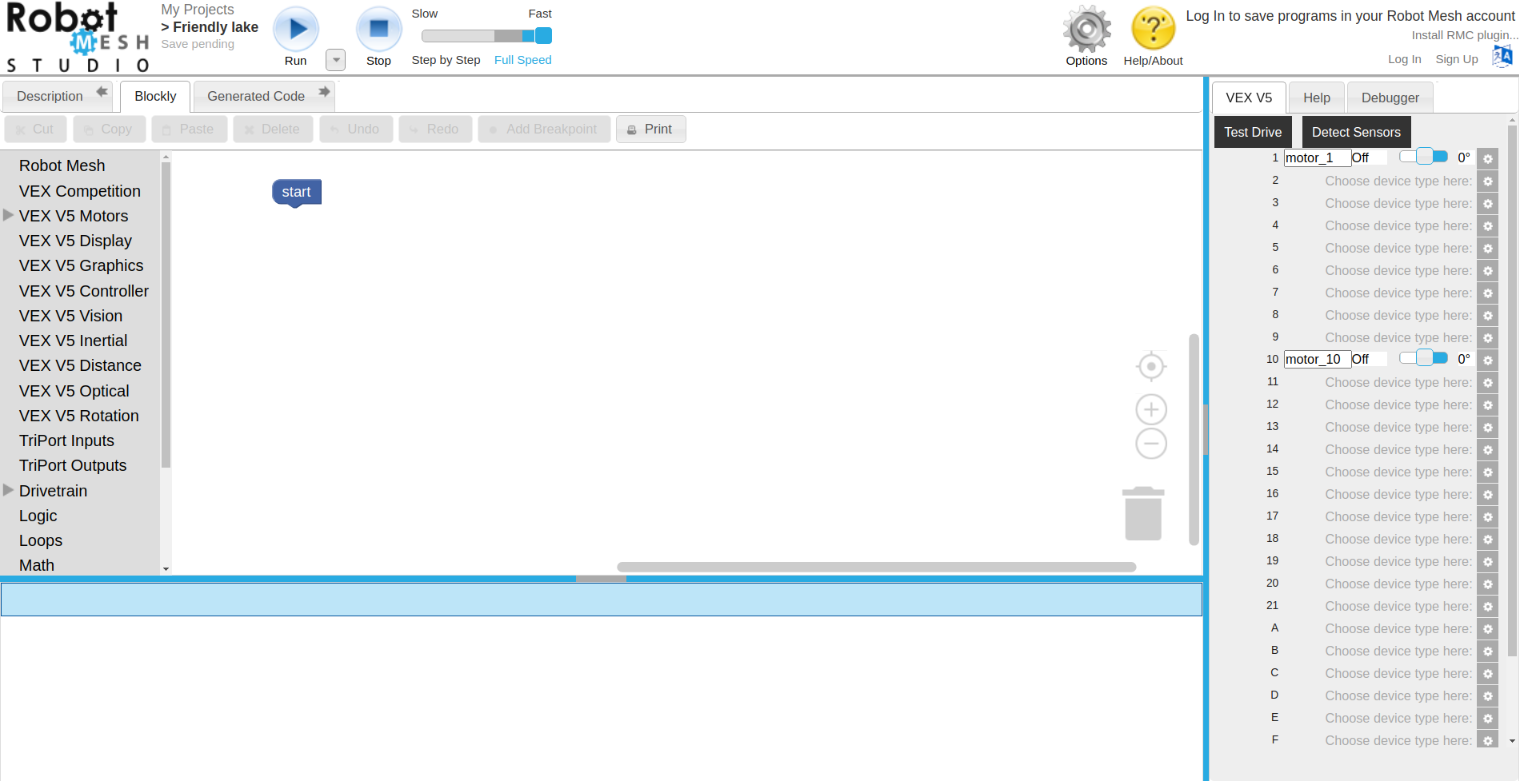
\includegraphics[width=\linewidth]{Images/01/add-motors-3.png}}%
			\caption{opakujte pro motor 10}%
		\end{subfigure}%
	\end{figure}

	\begin{question}
		Přiřaďte vašemu robotu motory. Nastavte jejich jména na \texttt{motor\_pravy} a \texttt{motor\_levy}.
	\end{question}

	\subsection{Náš první Blocky program}

	Programovací jazyk Blocky funguje na principu „bloků.“ Program vždy začíná v bloku \blockStartImage a poté pokračuje do bloku, který je pod tím, který právě dokončil. Jakmile dojdou bloky k vykonávání, tak~se program i robot zastaví.

	Pojďme naprogramovat základní program, který řekne robotovi, aby jel $3$ vteřiny dopředu:

	\begin{figure}[h!]
		\centering
		\begin{minipage}{0.5\textwidth}
			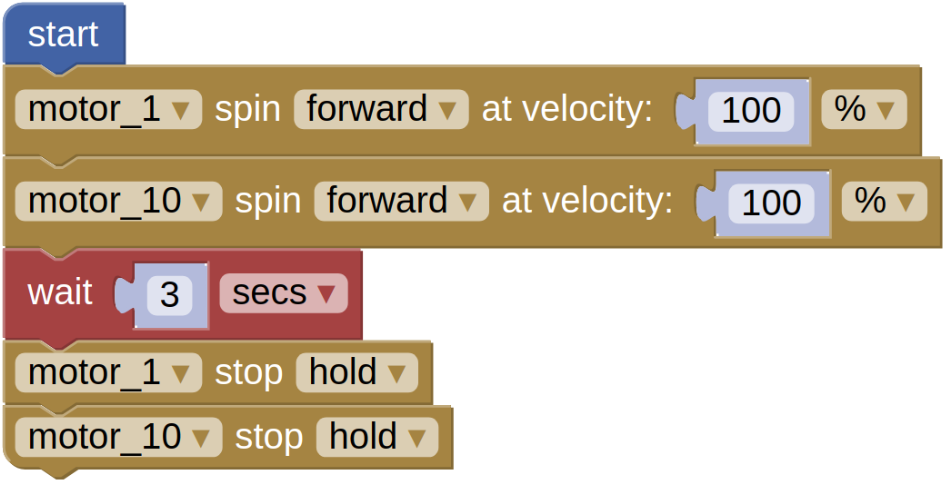
\includegraphics[width=\linewidth]{Images/01/program-1.png}
		\end{minipage}
	\end{figure}

	Vytvoříme ho tak, že v příkazové části klikneme na \textbf{VEX V5 Motors}, najdeme příkaz po startu a myší ho přetáhneme přímo pod start. Pro druhý rovněž opakujeme, ale motor (kliknutím) změníme na ten druhý. Příkaz \blockWaitImage najdeme v sekci \textbf{Robot Mesh}. Program spustíme tlačítkem \centerimage{2em}{Images/ui/play.png}.

	Robot se však místo toho, aby jel rovně, začal točit! To je kvůli tomu, že jeden motor je~\mbox{nainstalovaný} opačným směrem než ten druhý a „dopředu“ pro něj tedy znamená to, co pro druhý „dozadu.“ Pro~obrácený motor proto klikneme v hardwarové části na \centerimage{\baselineskip}{Images/ui/gear.png} a zaškrtneme \textbf{Reverse polarity}.

	Nyní zkusme spustit program znovu. Robot by měl správně jet dopředu.

	\subsubsection{Pozastavování a nahrávání}
	Kromě spouštění programů by se nám také hodilo program zastavit. Toho můžeme docílit tlačítkem \centerimage{2em}{Images/ui/stop.png}, které je napravo od tlačítka \centerimage{2em}{Images/ui/play.png}, nahoře v ovládací části.

	Pro testování pokročilejších programů se nám však může stát, že by se nám mohlo hodit program do robota pouze nahrát, a spustit to až po odpojení kabelu/nastavení robota. K tomu slouží tlačítko \centerimage{2em}{Images/ui/download.png}, které je dostupné kliknutím na \centerimage{\baselineskip}{Images/ui/dropdown.png}, nahoře v ovládací časti.

	\begin{question}
		Nahrajte tímto způsobem náš první program, robota odpojte a teprve poté ho přes jeho display spusťte.
	\end{question}

	\subsection{Programování virtuálního robota}
	Jedna z alternativ k programování reálného robota (toho doma každý k dispozici nemá...) je stránka \href{http://www.robotmesh.com/create/176384}{Hour of Code}, na které je možné programy psát a vykonávat na virtuálním robotovi v simulaci.

	\begin{figure}[h!]%
		\begin{subfigure}{.48\textwidth}%
			\centering%
			\fbox{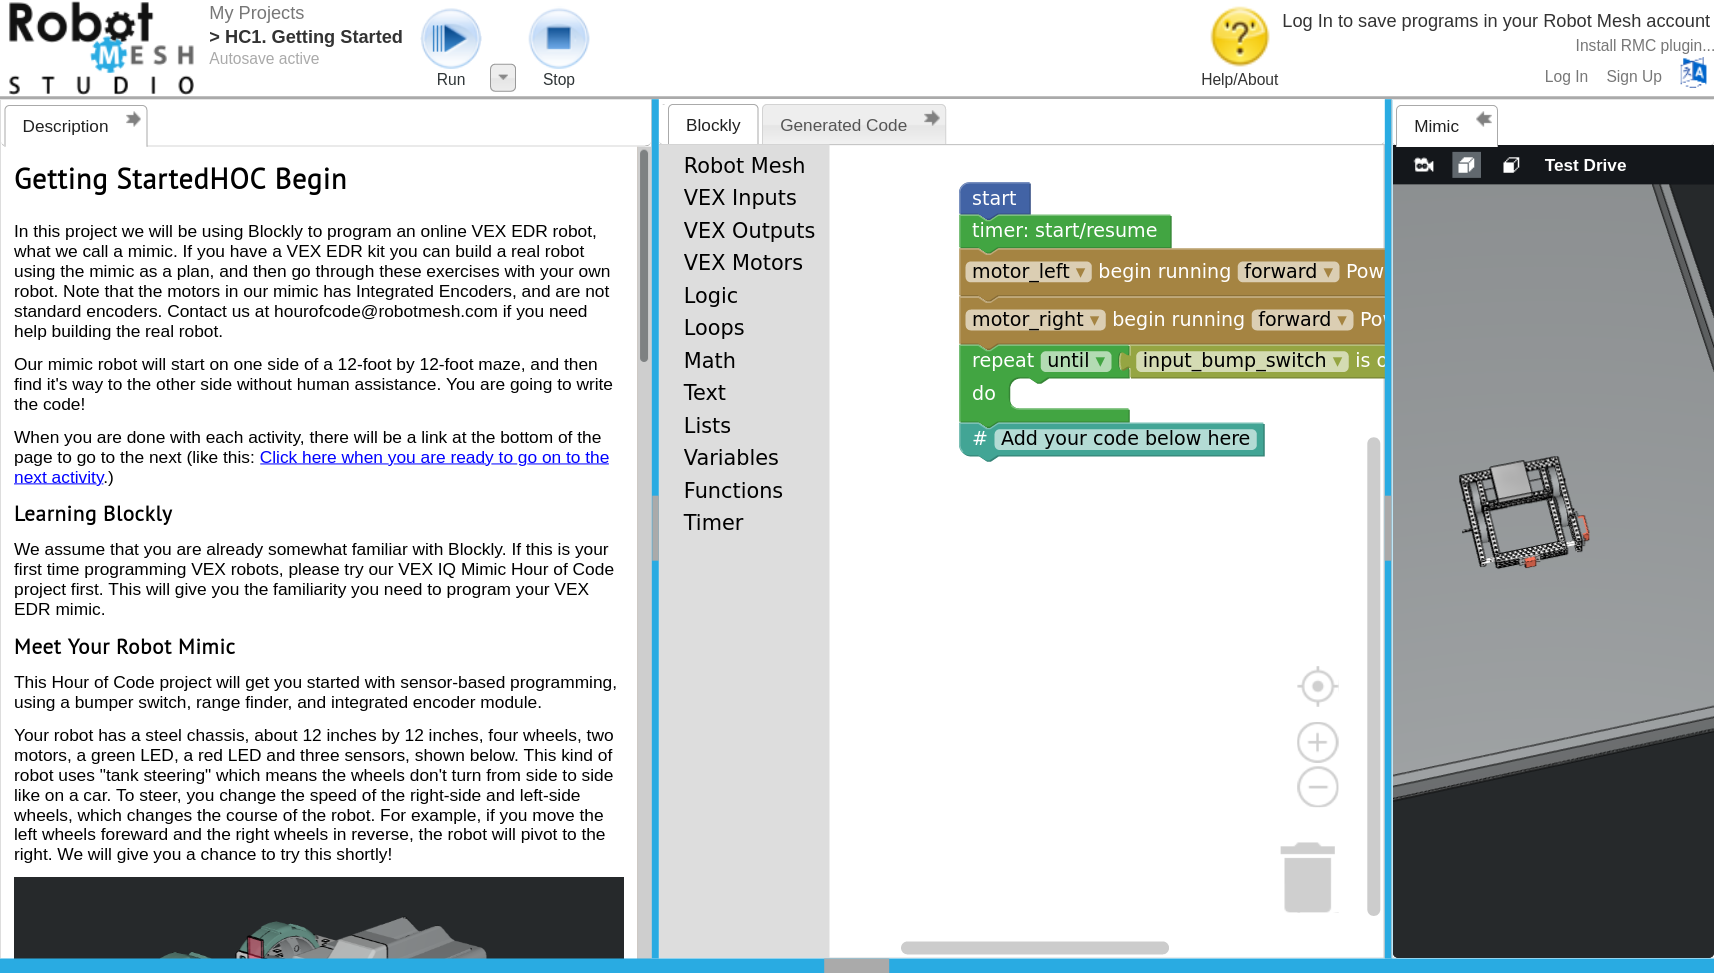
\includegraphics[width=\linewidth]{Images/01/hour-of-code.png}}%
			\caption{základní vzhled}%
		\end{subfigure} \hspace{.03\textwidth}%
		\begin{subfigure}{.48\textwidth}%
			\centering%
			\fbox{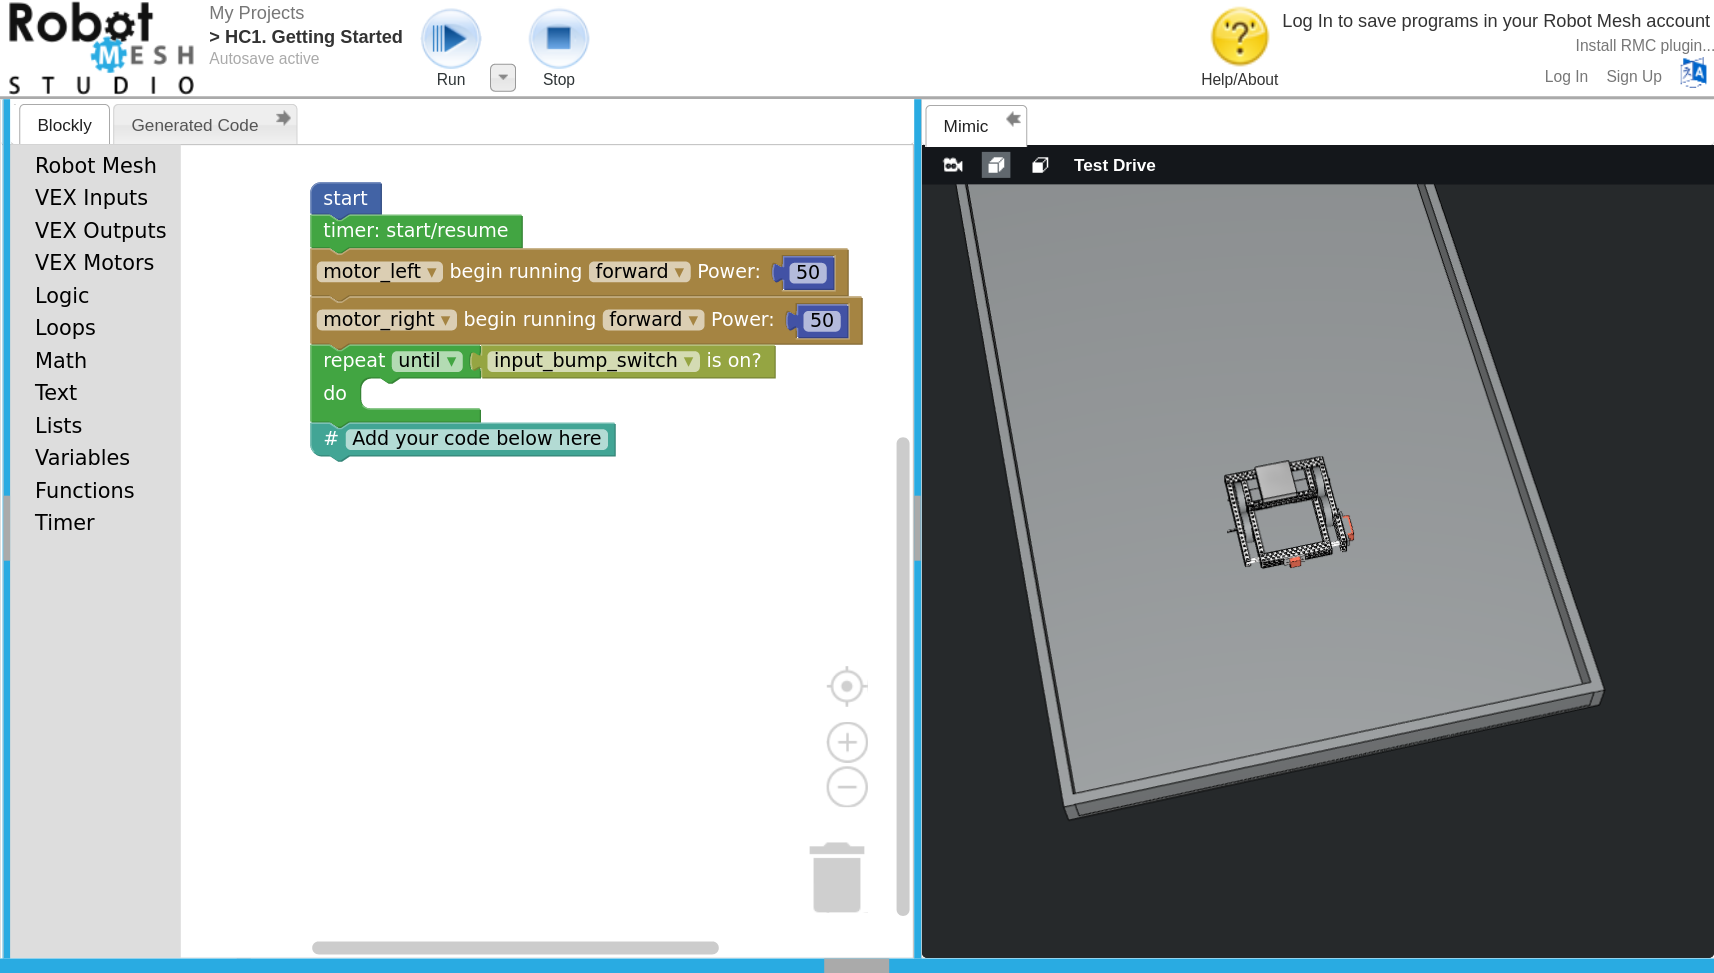
\includegraphics[width=\linewidth]{Images/01/hour-of-code-uimproved.png}}%
			\caption{vzhled po posunutí modrých oddělovačů}%
		\end{subfigure}%
		\caption{Stránka \href{http://www.robotmesh.com/create/176384}{Hour of Code}}
	\end{figure}

	Levou stranu s úvodem jde skrýt táhnutím modrého oddělovače, pravou se simulací jde obdobně rozšířit, aby se s robotem a programem lépe pracovalo. Je dobré si všimnout, že stránka neobsahuje hardwarovou část, protože není co nastavovat -- virtuální robot má motory a senzory již předdefinované (např. \texttt{motor\_left}, \texttt{motor\_right}).

	Je nutné doplnit, že se jedná o jiný typ robota, než ten, se kterým pracujeme. To ale pro cvičení psaní jednodušších programů v jazyce Blocky vůbec nevadí, protože většina základních konceptů probíraná v následujících kapitolách je identická.

	\begin{question}
		Spusťte přednastavený program. Co virtuální robot dělá?
	\end{question}

	\begin{solution}
		Robot je naprogramovaný tak, aby jel rovně do té doby, než narazí do zdi.
	\end{solution}

	\begin{question}
		Vytvořte a spusťte program z minulé části na virtuálním robotovi.
	\end{question}

\end{document}
